% Paper: refunding the token tax in speculative decoding for Hindi.
% Compiles with pdflatex + bibtex (e.g. upload the paper/ folder to Overleaf).
% Figures are in figures/; the bibliography is refs.bib.
\documentclass[11pt]{article}
\usepackage[margin=1in]{geometry}
\usepackage[T1]{fontenc}
\usepackage{times}
\usepackage{amsmath,amssymb}
\usepackage{booktabs}
\usepackage{graphicx}
\usepackage{xcolor}
\usepackage{natbib}
\usepackage[hidelinks]{hyperref}
\usepackage{caption}
\graphicspath{{figures/}}
\newcommand{\todo}[1]{\textcolor{red}{[TODO: #1]}}
\newcommand{\x}{$\times$}

\title{Refunding the Token Tax:\\
Cheap, Checked Drafting for Speculative Decoding in Hindi}
\author{Rakshit Sawarn (23b0426) \quad Kanika Sharma (23b2287) \\ Indian Institute of Technology Bombay \\ CS769 course project}
\date{}

\begin{document}
\maketitle

\begin{abstract}
Llama-3's tokenizer splits Hindi into 2.67 tokens per word, against 1.24 for English, and 59\% of
the tokens Llama-3-8B writes in Hindi only continue a word that has already started. In speculative
decoding, each of these tokens costs a full call of the draft model, although the draft predicts them
with 83--86\% accuracy. We measure how much of this \emph{token tax} can be refunded, and what collects
the refund. With an exact trace-based simulator for lossless speculative decoding (Llama-3-8B-Instruct
target, Llama-3.2-1B-Instruct draft, FLORES English$\to$Hindi), we show that free continuation tokens
would raise the speed-up from 1.45\x{} to 1.91\x: the refund lies in drafting cost, not in acceptance.
Trained word-completion heads on the draft model, with word-guided training and a lexicon filter,
collect a fifth of it (1.54\x). A training-free token 4-gram whose proposals the draft model checks
inside a call it makes anyway collects more than half (1.70\x), and the heads add nothing on top. On two
T4 GPUs the checked 4-gram is 1.62\x{} faster than decoding with the target alone, against 1.38\x{} for
the entropy baseline and 1.47\x{} for the best heads, with the target's output unchanged; our simulator
is within 1\% of the measured speed-ups. Most of the draft calls it saves (77\%) are on word
continuations. Word knowledge helps when proposals go to the target unchecked, but once the draft
model checks them, cheap coverage matters more than accuracy.
\end{abstract}

%=====================================================================
\section{Introduction}

Speculative decoding \citep{leviathan2023fast,chen2023accelerating} speeds up a large \emph{target}
model by letting a small \emph{draft} model propose several tokens that the target verifies in a
single forward pass. Because the target accepts exactly the tokens it would have produced itself, the
output is unchanged; the speed-up depends only on how many tokens are accepted per target pass and
how much drafting costs.

For languages that the tokenizer serves poorly, both quantities suffer. Hindi in Devanagari is split
by Llama-3's tokenizer into 2.67 tokens per word (Table~\ref{tab:tax}), so a Hindi sentence costs
more than twice as many decoding steps as its English translation. Recent work studies this
\emph{token tax} across 21 languages and finds that speculative decoding with built-in drafters gives
no refund for it: English gets the most tokens accepted per step, and tokens that continue a word are
only slightly easier to draft \citep{notokenrefund2026}.

We start from a different observation. In our setting the 1B draft model is \emph{very accurate
inside words}: it agrees with the 8B target on 83--86\% of word-continuation tokens, against about
66\% at word starts. The problem is not acceptance but price: each continuation token still costs a
full 1B forward pass (0.32 of an 8B step on our hardware). If the continuation tokens of a word could
be drafted almost for free, most of the tax would be refunded.

We first size this refund and then test two ways to collect it. The natural idea is to teach the draft
model to complete words cheaply: small multi-token heads on its hidden state, trained to predict the
rest of the current word, optionally constrained by a Hindi lexicon. These help, but the heads are far
less accurate than the draft itself, and each wrong proposal costs a round. The second idea needs no
training: a cheap source (a token n-gram) proposes the next tokens, and the draft model checks them in
the forward pass it makes anyway, so only tokens the draft agrees with reach the target. This is the
vertical cascade of \citet{chen2024cascade}; we do not claim the mechanism, but show why it fits a
high-fertility language and how it compares with trained, word-aware proposers.

\paragraph{Contributions.}
\begin{enumerate}
  \item \textbf{The refund is large and lies in drafting cost.} With an exact trace-based simulator
  we show that free continuation tokens of draft-model quality would raise the lossless speed-up from
  1.452\x{} to 1.911\x{}. Dictionary completers lack the context to collect it unchecked.
  \item \textbf{Checked drafting collects more than half of it, without training.} A token 4-gram
  checked by the draft model reaches 1.701\x{} in simulation and 1.620\x{} on hardware (Entropy:
  1.384\x). 77\% of the draft calls it saves are on word continuations, and its gain grows with the
  share of continuation tokens in a sentence.
  \item \textbf{Trained word-completion heads lose.} Heads with word-guided training and a lexicon
  filter are the best unchecked proposers (1.542\x{} simulated, 1.469\x{} on hardware), but stay well
  below the checked 4-gram and add nothing on top of it. Word knowledge (training, lexicon, word tries)
  pays off when proposals are unchecked and matters little once they are checked.
  \item \textbf{A validated simulator.} A real decoding loop on two T4 GPUs reproduces the simulated
  speed-ups within 1\% for every drafter.
\end{enumerate}

%=====================================================================
\section{Background and related work}
\label{sec:related}

\paragraph{Speculative decoding and decoding heads.}
Medusa \citep{cai2024medusa} adds extra heads to the target's last hidden state, each predicting a
token further ahead; Hydra \citep{ankner2024hydra} makes the heads sequentially dependent.
Multi-token prediction is also used as a training objective \citep{gloeckle2024better}. Our
word-completion heads are Medusa-1 style, but on the \emph{draft} model, trained only on positions
inside words, and used as a cheap supplement to the draft's own LM head rather than a replacement for it.

\paragraph{Retrieval and dictionary drafters.}
REST \citep{he2024rest} and SuffixDecoding \citep{oliaro2024suffixdecoding} draft from a datastore
or suffix tree. DictSpec \citep{dictspec2026} drafts Ukrainian and Crimean Tatar from a static
n-gram table, with gains that grow with tokenizer fertility, and \citet{paudel2026ngram} find that
n-gram drafters give moderate speed-ups across languages because drafting with them costs almost
nothing. Our dictionary baselines test this idea for Hindi and quantify its limit. These drafters
propose directly to the target; in checked drafting (Section~\ref{sec:checked}) an n-gram's proposals
are first checked by the draft model.

\paragraph{Cascaded drafting.}
Staged speculative decoding \citep{spector2023staged} adds a cheaper second draft stage below the draft
model, a Katz back-off trigram model. Cascade Speculative Drafting \citep{chen2024cascade} generalises
this into a \emph{vertical cascade}, in which each draft model reviews the drafts of a smaller one down
to a statistical model (Max-Gram: longest matches with the prompt or the generation so far, with a
bigram fallback), and combines it with a \emph{horizontal cascade} that uses smaller drafters for later
tokens. Our checked drafting is a vertical cascade with a token n-gram at the bottom; we do not claim the
mechanism. We add an account of why it works for a high-fertility language (most of the draft calls it
saves are word continuations), and a controlled comparison, in simulation and on hardware, with trained
word-completion heads and lexicon constraints, which it beats.

\paragraph{Adaptive drafting.}
Several systems switch between drafters or stop drafting based on confidence
\citep[e.g.][]{respec2026,talon2026,metasd2025}. Our unchecked heads use a linguistic switch (the draft
model writes word starts, the heads continue words); in checked drafting the draft model decides, token
by token, which cheap proposals to keep.

\paragraph{Indic languages.}
\citet{naidu2026phrase} trains phrase-level heads on a frozen target. Its Hindi speed-ups are
2.09\x{} on Gemma-3-1B and 1.49\x{} on Gemma 4 E2B, but 1.29\x{} on Qwen3-4B, whose tokenizer needs
about five tokens per Hindi word against 1.5 for Gemma-3. We study another tokenizer with a high token
tax (Llama-3), put our heads on the draft model instead of the target, and compare them with
training-free checked drafting.

\paragraph{Our Phase 1.} In earlier work on the same setting we tried to decide \emph{when to stop
drafting} using word and morpheme boundaries. None of the linguistic stopping rules beat a plain
entropy rule, which is therefore our baseline. We also tried a universal word-level head that reads the
text so far and the target's top candidates as strings, and is trained on the outputs of other LLMs;
applied zero-shot to the 8B it reached 1.296\x{} [1.287, 1.306], well below the entropy rule.

%=====================================================================
\section{Setup and cost model}
\label{sec:setup}

\paragraph{Models and data.} Target: Llama-3-8B-Instruct; draft: Llama-3.2-1B-Instruct; both in
fp16. The target is split over two NVIDIA T4 GPUs, so every target step includes a transfer between
GPUs; the draft runs on one of them. Task: English$\to$Hindi translation of FLORES-200 \citep{nllb2022}; we tune all
hyperparameters on \emph{dev} and report on \emph{devtest} (1{,}012 sentences). For every sentence we
record the target's greedy output $y$ and, at every position $t$, the draft model's distribution given
$y_{<t}$ (teacher forcing).

\paragraph{Exact simulation.} Because verification is lossless and greedy, a drafted token $y'_t$ is
accepted iff it equals $y_t$ and all earlier drafted tokens in the round were accepted. Given the
recorded draft predictions along $y$, the number of accepted tokens in each round, and therefore the
sequence of committed tokens, can be computed exactly without running the models. Only the number of
further tokens drafted after a wrong one is approximate, because it uses draft features along $y$; in
Phase 1 this changed the speed-up by 0.2--1.4\%. In total, a real GPU decoding loop was 3.4--7.8\% below
the Phase 1 simulation on 100 sentences (Entropy: 1.440\x{} simulated, 1.356\x{} real). The decoding
loop of Section~\ref{sec:real} removes most of the loop overhead: there, the simulation is within 1\% of
the measured speed-up for every drafter.

\paragraph{Cost.} We measure time in units of one target forward. A draft call costs
$c = t_\text{draft}/t_\text{target} = 0.323$. Verifying $g$ drafted tokens costs
$v(g) = t_\text{verify}(g)/t_\text{target}$, measured for $g\le 8$ (1.02 to 1.07). Reading $q$
pending tokens into the draft's KV cache in one call costs $c\,r(q)$ with $r(q)\approx 1$ for $q \le 8$
(measured with LM-head logits at every position read). A forward of the $K=3$ heads over the continuation vocabulary costs $0.018\,c$; over the
full 128k vocabulary it costs $0.114\,c$. The speed-up on a set of sentences is
\begin{equation}
S = \frac{\sum_\text{rounds} (a + 1)}{\sum_\text{rounds} \big(C_\text{draft} + v(g)\big)},
\end{equation}
where $a$ is the number of accepted drafted tokens in a round (the target always adds one token).
Confidence intervals are 95\% bootstrap intervals over sentences; differences between two
systems use a paired bootstrap.

\paragraph{Entropy baseline.} The draft keeps drafting while
$1-\sqrt{\beta H_t} \ge \lambda$, where $H_t$ is its predictive entropy ($\beta=4$, at most 8 tokens
per round, $\lambda$ tuned). This gives 1.452\x{} [1.444, 1.461], with 2.48 tokens per target call.

%=====================================================================
\section{How much tax can be refunded?}
\label{sec:feasibility}

\paragraph{Ceiling.} Suppose every word-continuation token could be drafted at a cost $\kappa c$ with
exactly the draft model's prediction. With $\kappa=0$ the speed-up is 1.946\x; with $\kappa = 0.05$
it is 1.911\x{} [1.894, 1.931], a potential gain of $+0.46$ over Entropy. The refund is thus in the
cost of drafting, not in acceptance.

\paragraph{Break-even accuracy.} A cheap completer that proposes directly to the target is less
accurate than the draft. If it keeps a share $\rho$ of the draft's correct continuation tokens (and
always proposes), the speed-up falls roughly linearly (Figure~\ref{fig:rho}) and reaches the entropy
baseline at $\rho\approx0.7$.

\paragraph{Dictionaries lack context.} Table~\ref{tab:ctx} measures whole-word completion accuracy
at 38.7k mid-word positions. A prefix dictionary built from 72.8k Hindi word types completes 31\% of
words correctly; adding the previous word and a sentence cache gives 35\%; even adding the words of
the reference translation (an oracle) gives only 47\%. The draft model gets 77\%. Used at every
mid-word position the dictionary drafter is far worse than Entropy (1.226\x); used only when its top
completion is dominant (at least 60\% of the frequency mass of matching words) it gains a little,
1.471\x{} [1.462, 1.480]. Unchecked, a completer must be accurate; Section~\ref{sec:checked} shows that
this requirement disappears once the draft model checks the proposals.

\begin{table}[t]
\centering
\begin{tabular}{lr}
\toprule
completer & whole-word accuracy \\
\midrule
dictionary, prefix only & 31.3\% \\
\quad + previous word (bigram) + sentence cache & 34.9\% \\
\quad + words of the reference translation (oracle) & 47.3\% \\
1B draft model & \textbf{77.2\%} \\
\bottomrule
\end{tabular}
\caption{Completing the current word from its first token(s), 38.7k mid-word positions of the 8B's
FLORES devtest outputs.}
\label{tab:ctx}
\end{table}

\begin{figure}[t]
\centering
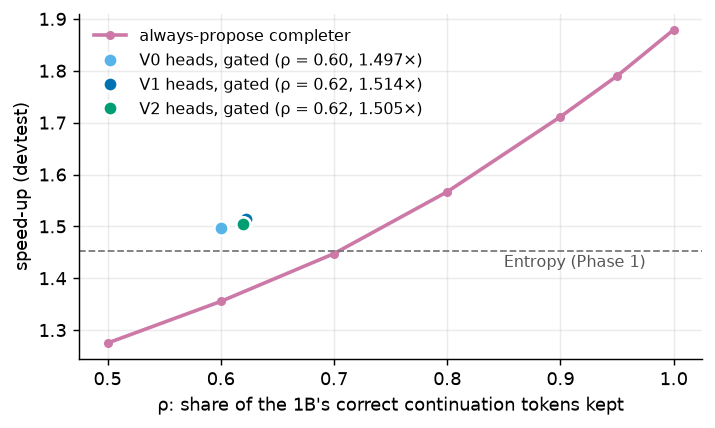
\includegraphics[width=0.7\linewidth]{fig_rho.png}
\caption{Speed-up of an always-proposing, unchecked completer that keeps a share $\rho$ of the draft
model's correct continuation tokens. Break-even with Entropy is at $\rho\approx0.7$. The
confidence-gated heads of Section~\ref{sec:method} lie above the curve.}
\label{fig:rho}
\end{figure}

%=====================================================================
\section{Unchecked proposers: word-completion heads}
\label{sec:method}

\paragraph{Architecture.} Let $h_t$ be the draft model's last hidden state that predicts $y_t$. We add
$K=3$ Medusa-1 heads $z_k = h_t + \mathrm{SiLU}(W_k h_t)$ ($W_k$ zero-initialised) followed by the
frozen, shared LM head of the 1B; head $k$ predicts $y_{t+k}$. At inference the LM head is restricted
to the \emph{continuation vocabulary}: the 1{,}406 Llama-3 tokens without a leading space or
word-initial marker, which cover 96.3\% of the target's continuation tokens. This reduces the cost of a
head from about a quarter of a draft call to under 2\%. A \emph{continuation head}
$\mathrm{Linear}(d, K)$ predicts whether $y_{t+1..t+k}$ all continue the current word.

\paragraph{Training.} The 1B is frozen. We train with teacher forcing on filtered IITB English--Hindi
pairs \citep{kunchukuttan2018iitb} using the same translation prompt (batch 32, learning rate
$10^{-3}$): 60k pairs (1{,}867 steps, 31 minutes on a T4) and, to test data scaling, 180k pairs (5{,}598
steps, 1.8 hours). One draft forward per batch trains three variants on identical data:
\textbf{V0} (plain MTP) uses $\sum_k 0.8^{k-1}\,\mathrm{CE}_k$ at every position; \textbf{V1}
(word-guided) uses $\mathrm{CE}_k$ only where $y_{t+1..t+k}$ continue the current word, plus
$0.5\cdot\mathrm{BCE}$ for the continuation head; \textbf{V2} combines V1's losses with learned
uncertainty weights \citep{kendall2018multi}.

\paragraph{Drafting.} In each round the draft model drafts a token with its own LM head. If that token
contains Devanagari (or is a fragment of a Devanagari character) and the entropy rule does not stop the
round, the heads propose up to $K$ continuation tokens, stopping at head confidence below $\tau_h$ or
(V1/V2) continuation probability below $\tau_c$. The proposed tokens go to the target \emph{unchecked};
the next draft call reads them in one forward (cost $c\,r(1+q)$). \emph{Lexicon filter:} proposals also
stop as soon as the current word is no longer a prefix of a word in a 72.8k-type lexicon (dev target
outputs and a public Hindi word list), a CPU binary search. All thresholds and $\lambda$ are tuned on
dev by coordinate search.

\subsection{Results}
\label{sec:results}

\begin{table}[t]
\centering
\small
\begin{tabular}{lccc}
\toprule
drafter & 60k pairs & 180k pairs [95\% CI] & $\Delta$ vs.\ Entropy, 180k \\
\midrule
Entropy & \multicolumn{2}{c}{1.452 [1.444, 1.461]} & --- \\
Dictionary, every mid-word position & \multicolumn{2}{c}{1.226 [1.218, 1.234]} & $-0.226$ \\
Dictionary, confidence-gated & \multicolumn{2}{c}{1.471 [1.462, 1.480]} & $+0.019$ \\
\midrule
Heads V0, plain MTP & 1.497 & 1.510 [1.500, 1.522] & $+0.059$ \\
Heads V1, word-guided & 1.514 & 1.518 [1.508, 1.530] & $+0.066$ \\
Heads V2, adaptive weights & 1.505 & 1.517 [1.507, 1.529] & $+0.065$ \\
Heads V0 + lexicon filter & 1.529 & 1.538 [1.525, 1.551] & $+0.086$ \\
\textbf{Heads V1 + lexicon filter} & 1.533 & \textbf{1.542 [1.530, 1.555]} & $\mathbf{+0.090}$ [$+0.084$, $+0.097$] \\
\midrule
Ceiling: free continuations ($\kappa=0.05$) & \multicolumn{2}{c}{1.911 [1.894, 1.931]} & $+0.459$ \\
\bottomrule
\end{tabular}
\caption{Unchecked proposers, simulated lossless speed-up on FLORES devtest (1{,}012 sentences),
tuned on dev. Heads use the continuation vocabulary; columns give the heads' training data.}
\label{tab:main}
\end{table}

\paragraph{Heads collect a fifth of the refund.} Table~\ref{tab:main} gives the results. Every head
variant beats Entropy and the gated dictionary; the best unchecked system, V1 heads with the lexicon
filter, reaches 1.542\x{} with the 180k heads, $+0.090$ of the $+0.459$ available. On hardware it gives
1.469\x{} against 1.384\x{} for Entropy (Section~\ref{sec:real}). The heads are far less accurate than
the draft model (V1, 180k: 57.2/49.8/43.9\% on continuation tokens at distances 1--3, V0:
55.5/42.8/32.7\%, draft: 83--86\%) and keep only about 65\% of the draft's correct first continuations,
below the break-even of Figure~\ref{fig:rho}. They still win because they propose only when confident.
Full-vocabulary heads, and re-ranking their top-8 with the lexicon, are no better and cost six times more.

\paragraph{Word knowledge helps, but only once.} Word-guided training beats plain MTP: V1 $-$ V0 is
$+0.016$ [$+0.012$, $+0.020$] with 60k pairs and $+0.008$ [$+0.004$, $+0.012$] with 180k, since plain
heads gain more from data; word guidance is partly a data-efficiency aid. Uncertainty weighting (V2)
does not help. The lexicon filter adds $+0.024$ [$+0.019$, $+0.029$] to V1 (180k), and lets the tuned
system propose more (2.67 vs.\ 2.48 tokens per target call). With the filter on, V1 and V0 are tied
with 60k pairs ($+0.004$ [$-0.001$, $+0.009$]) and nearly tied with 180k ($+0.005$ [$+0.001$, $+0.009$]):
the lexicon supplies the knowledge of where a word may end that V1 otherwise learns. Tripling the
training data gains only $+0.010$ [$+0.006$, $+0.013$] for the best system, so more data will not close
the gap to the ceiling.

% Checked drafting: method, simulated results, analyses. Included from main.tex.
% Numbers: results/checked/{main_table.csv, wordtrie.csv, where_saved.json, gain_by_share.csv, extra.json}
% (scripts/run_checked_sim.py, scripts/feasibility/checked_wordtrie.py, scripts/checked_analysis.py).
%=====================================================================
\section{Checked drafting}
\label{sec:checked}

The heads of Section~\ref{sec:method} append their proposals to the draft unchecked, so a wrong head
token reaches the target and ends the round. Yet the draft model reads those proposals anyway in its
next call (cost $c\,r(1+q)$ with $r\approx1$), and that forward also gives the draft's own prediction
after every token it reads. Checked drafting uses this to filter proposals before the target sees them.

\paragraph{Mechanism.} A draft call reads the pending token together with a proposal
$F=(f_1,\dots,f_q)$ and computes its argmax $\hat y_1,\dots,\hat y_{q+1}$ at all $q+1$ positions. It keeps
the longest prefix $f_1,\dots,f_m$ with $f_j=\hat y_j$, appends its own next token $\hat y_{m+1}$, and
crops the rejected proposal tokens from its KV cache. Every drafted token is therefore the draft's own
greedy token: the chain offered to the target is the one plain drafting would produce, but $m$ of its
tokens cost no draft call of their own. The entropy rule is evaluated on the last token of each call and
only decides whether another call is made; tokens a call has already produced are kept. The cost
$r(q)$ was measured with LM-head logits at every position read, so scoring the proposal is included.
The target verifies as before and the output is unchanged. This is the \emph{vertical cascade} of
\citet{chen2024cascade} and \citet{spector2023staged}, with our 1B as the reviewing draft
(Section~\ref{sec:related}).

\paragraph{Proposal sources.}
\begin{itemize}
  \item \textbf{4-gram.} A token 4-gram from 190k IITB Hindi sentences (10.5M Llama-3 tokens): the
  most frequent next token after the longest context (four tokens down to one) seen at least twice,
  applied greedily for up to $L$ tokens. The table takes 6\,MB and a lookup 0.05\,ms on the CPU,
  against 23\,ms for a draft call. It needs no training and knows nothing about words.
  \item \textbf{Heads.} The continuation-vocabulary chain of V0 or V1, read from the hidden state of the
  last token of the previous call and cut at head probability $\tau_h$; the first call of a round has no
  head proposal. The Devanagari gate and the head cost ($0.018\,c$ per call) are as in
  Section~\ref{sec:method}.
  \item \textbf{Both.} The heads' tokens, extended by the 4-gram to $L$ tokens.
\end{itemize}
$\lambda$, $L\in\{4,6,7\}$ and $\tau_h$ are tuned on dev. As further proposers we test a word trie
built from the same corpus, which completes the current word (optionally conditioned on the previous
word, and also proposing the most frequent next word), and, as a bound, the rest of the word the draft
itself will write.

\paragraph{Simulation.} The recorded draft argmax along $y$ tells which proposal tokens the draft
accepts, so rounds and draft calls are exact while the draft is on the target's path. After a wrong
draft token we propose nothing and charge a full call per further token, which is conservative (those
tokens are rejected anyway). Section~\ref{sec:real} tests the simulation against a real decoding loop.

\begin{table}[t]
\centering
\small
\begin{tabular}{lcc}
\toprule
drafter & speed-up [95\% CI] & $\Delta$ vs.\ Entropy [95\% CI] \\
\midrule
Entropy & 1.452 [1.444, 1.461] & --- \\
Heads V1 + lexicon filter, unchecked & 1.542 [1.530, 1.555] & $+0.090$ [$+0.084$, $+0.097$] \\
\midrule
\multicolumn{3}{l}{\emph{checked by the draft model:}} \\
Heads V0 & 1.568 [1.556, 1.581] & $+0.116$ [$+0.112$, $+0.121$] \\
Heads V1 & 1.572 [1.560, 1.586] & $+0.120$ [$+0.115$, $+0.125$] \\
Word trie, current word & 1.582 [1.570, 1.594] & $+0.130$ [$+0.126$, $+0.134$] \\
Word trie + previous word + next word & 1.659 [1.646, 1.673] & $+0.207$ [$+0.202$, $+0.213$] \\
\textbf{4-gram (no training)} & \textbf{1.701 [1.687, 1.716]} & $\mathbf{+0.249}$ [$+0.242$, $+0.256$] \\
4-gram + heads V0 & 1.708 [1.694, 1.724] & $+0.257$ [$+0.249$, $+0.264$] \\
4-gram + heads V1 & 1.705 [1.690, 1.720] & $+0.253$ [$+0.246$, $+0.260$] \\
\midrule
Bound: the draft's own word completion & 1.857 [1.841, 1.875] & $+0.406$ [$+0.395$, $+0.415$] \\
Ceiling: free continuations ($\kappa=0.05$) & 1.911 [1.894, 1.931] & $+0.459$ [$+0.449$, $+0.470$] \\
\bottomrule
\end{tabular}
\caption{Checked drafting, simulated on FLORES devtest (1{,}012 sentences), tuned on dev. The
unchecked heads are the best system of Section~\ref{sec:results}. Heads trained on 180k pairs. The
bound proposes the rest of the word the draft itself will write. $\Delta$: paired bootstrap.}
\label{tab:checked}
\end{table}

\paragraph{Being checked matters more than the proposer.} Table~\ref{tab:checked} gives the results.
Checking alone lifts the V1 heads above the paper's best unchecked system (V1 + lexicon filter) by
$+0.030$ [$+0.024$, $+0.035$]. The training-free 4-gram is far ahead of every head system: $+0.159$
[$+0.151$, $+0.166$] over V1 + lexicon and $+0.129$ [$+0.123$, $+0.135$] over checked V1 heads. On top
of the 4-gram, heads add only $+0.008$ [$+0.006$, $+0.009$] (V0) or $+0.004$ [$+0.002$, $+0.006$] (V1),
and nothing at all on hardware (Section~\ref{sec:real}). Word tries, whose proposals are always real
words, also stay below the 4-gram. Once the draft model checks every proposal, a wrong proposal costs
almost nothing, so what counts is how much a proposer covers, not how often it is right: in the real
loop the 4-gram proposes 8.8 tokens per round and the draft accepts 10\% of them, while the checked V1
heads propose 2.3 tokens per round and the draft accepts 22\%. The heads propose at most $K=3$
continuation tokens inside a word and not at the first call of a round; the 4-gram proposes up to seven
tokens, across word boundaries. Word knowledge (V1's training, the lexicon, a word trie) pays off when
proposals are unchecked, where a wrong token is expensive, and matters little once they are checked.
The bound in Table~\ref{tab:checked} (1.857\x) shows that better proposers could still gain.

\paragraph{The saved calls are word continuations.} Of the draft calls that the 4-gram saves, 77.4\%
are on word-continuation tokens, although only 59.4\% of all tokens, and 64.8\% of the tokens the draft
predicts correctly, are continuations. The gain also grows with how taxed a sentence is
(Figure~\ref{fig:checked_share}): over devtest quintiles of continuation-token share, the gain over
Entropy rises from 14.5\% to 18.8\% (19.1\% in the fourth quintile; Spearman $\rho=0.21$). The same
analysis for V1 + lexicon gives 5.5\% to 8.2\% ($\rho=0.14$). The 4-gram mostly collects the refund of
Section~\ref{sec:feasibility}: once a word has started, its continuation is easy to guess, and the draft
confirms the guess in a call it makes anyway.

\begin{figure}[t]
\centering
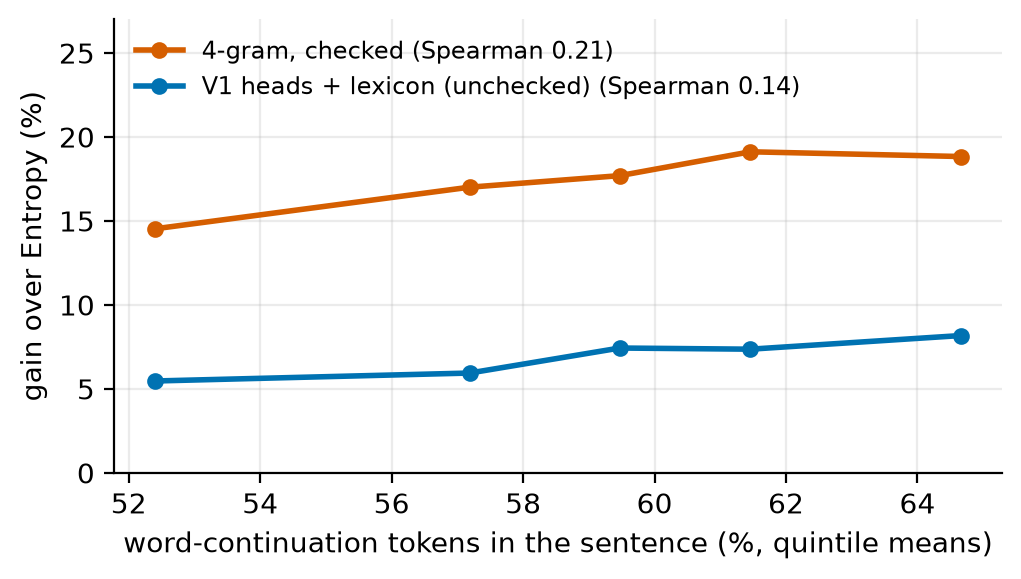
\includegraphics[width=0.7\linewidth]{fig_checked_share.png}
\caption{Gain over Entropy by sentence continuation-token share (devtest quintiles, simulated).}
\label{fig:checked_share}
\end{figure}

\paragraph{Little data, robust to overhead.} The 4-gram needs little data
(Figure~\ref{fig:checked_data_cost}, left): 1k sentences already give 1.615\x, and a 4-gram from only
the 997 dev outputs of the target, without any external corpus, gives 1.660\x. If a call that reads a
proposal cost 5, 10 or 20\% more than measured, the 4-gram would still reach 1.677\x, 1.654\x{} and
1.610\x{} (Figure~\ref{fig:checked_data_cost}, right), above every unchecked head system. The real loop
shows that the measured cost holds.

\begin{figure}[t]
\centering
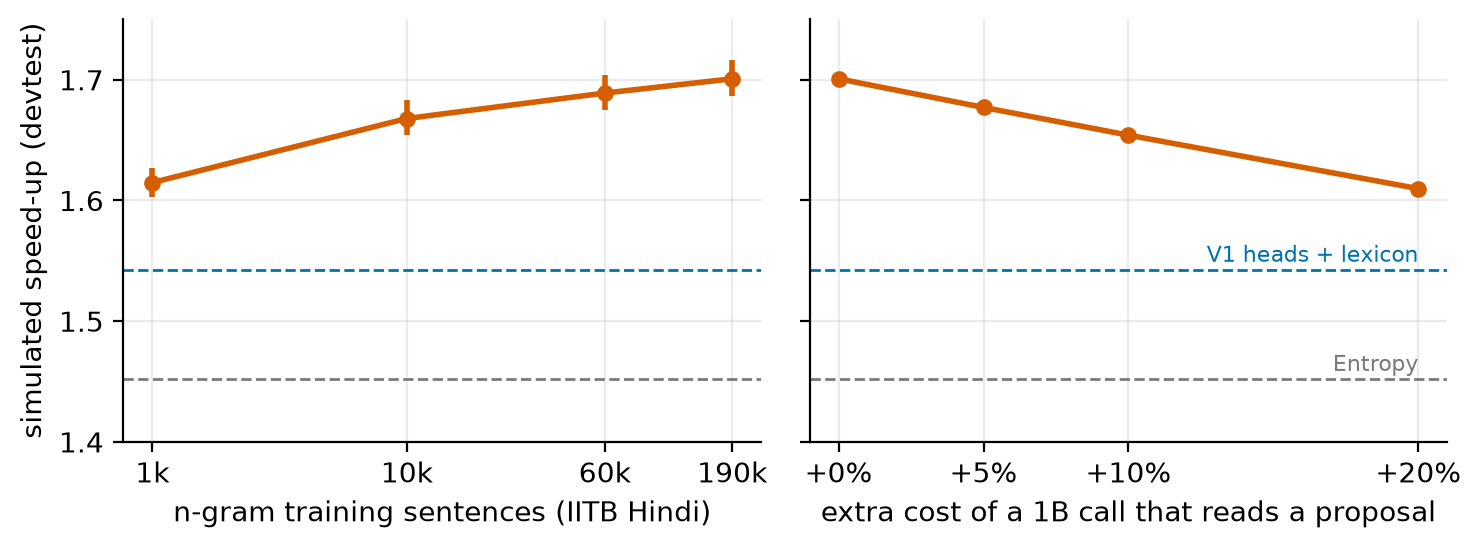
\includegraphics[width=0.9\linewidth]{fig_checked_data_cost.png}
\caption{Checked 4-gram, simulated devtest speed-up. Left: n-gram training sentences (95\% CIs).
Right: extra cost of a draft call that reads a proposal. Dashed: Entropy and V1 heads + lexicon filter.}
\label{fig:checked_data_cost}
\end{figure}

% Real decoding loop on GPUs. Included from main.tex.
% Numbers: results/heads_loop/{SUMMARY.md, summary.json, paired_wall.json, sim_vs_real.csv},
% results/checked/extra.json (kaggle/09_heads_loop.ipynb, scripts/checked_analysis.py).
%=====================================================================
\section{Real decoding on GPUs}
\label{sec:real}

\paragraph{Setup.} All drafters run in one decoding loop (batch size 1, KV caches for target and draft,
fp16, Hugging Face Transformers 5.22, PyTorch 2.11), timed on Kaggle with two T4 GPUs and the target
split over both as in Section~\ref{sec:setup}. We decode the same 100 devtest sentences as the Phase-1
loop, up to 256 new tokens, three times each; within a repeat the methods run in a rotating order per
sentence. All thresholds are the dev-tuned values from simulation (180k heads); nothing is tuned on the
real loop. The speed-up is the ratio of the sums over sentences of the median wall-clock time over
repeats, relative to NoDraft (greedy decoding with the target alone, in the same loop); \emph{decode
only} excludes the target's prompt prefill, which the simulation does not model. Compared with the
Phase-1 loop, drafting stops at an end-of-text token, NoDraft never runs the draft model, the draft
reads the prompt in its first draft call, and LM-head logits are computed only where they are needed;
these changes apply to every method.

\begin{table}[t]
\centering
\small
\setlength{\tabcolsep}{4pt}
\begin{tabular}{lccccc}
\toprule
drafter & wall-clock [95\% CI] & decode only & sim. & tokens/round & calls/round \\
\midrule
NoDraft & 1.000 & 1.000 & --- & 1.00 & 0.00 \\
Entropy & 1.384 [1.359, 1.408] & 1.395 & 1.409 & 2.45 & 2.08 \\
V1 + lexicon filter & 1.469 [1.433, 1.504] & 1.483 & 1.497 & 2.63 & 2.10 \\
V1, checked & 1.505 [1.467, 1.539] & 1.520 & 1.520 & 2.55 & 1.84 \\
\textbf{4-gram, checked} & \textbf{1.620 [1.580, 1.657]} & \textbf{1.640} & 1.641 & 2.54 & 1.48 \\
4-gram + V0, checked & 1.620 [1.581, 1.657] & 1.640 & 1.650 & 2.54 & 1.45 \\
\bottomrule
\end{tabular}
\caption{Real decoding loop on two T4 GPUs: 100 FLORES devtest sentences, 3 repeats, speed-up over
NoDraft. V0/V1: heads trained on 180k pairs. \emph{sim.}: the simulator on the same 100 sentences with
the costs measured in the same session ($c=0.333$), to be compared with \emph{decode only}.
Tokens/round: tokens committed per target call; calls/round: draft calls per round.}
\label{tab:real}
\end{table}

\paragraph{The ranking holds on hardware.} Table~\ref{tab:real} gives the results. The checked 4-gram is
the fastest drafter: $+0.236$ [$+0.218$, $+0.254$] over Entropy (17\% faster), $+0.151$ [$+0.129$,
$+0.174$] over V1 + lexicon and $+0.115$ [$+0.099$, $+0.132$] over checked V1 heads (paired, wall-clock).
Checking also helps the heads: $+0.036$ [$+0.020$, $+0.053$] over V1 + lexicon. Heads on top of the
4-gram add $+0.000$ [$-0.005$, $+0.005$]. Every method reproduces the target's unbatched greedy output
in 96\% of decodes, the same share as NoDraft; the other decodes (four sentences) differ through fp16
numerical near-ties, as in Phase 1.

\paragraph{The simulation is accurate.} On the same sentences and with the costs measured in the same
session, the simulated speed-up is within 1\% of the measured decode-only speed-up for every method
($-1.0\%$ to $+0.0\%$), and tokens per target call agree within 0.01. With the Phase-1 cost measurement
($c=0.323$) the gap is 1.7--2.8\%, so most of the remaining difference is session-to-session variation
of the measured costs; the 3.4--7.8\% gap of Phase 1 came from loop overheads that the new loop removes.
The real loop needs slightly fewer draft calls than simulated (1.48 vs.\ 1.51 per round for the 4-gram)
because it keeps proposing after a wrong draft token, where the simulation charges a full call.

\paragraph{Costs on hardware.} A draft call took 23.3\,ms whether it read one token (Entropy) or a
proposal of up to eight (4-gram), which confirms $r(q)\approx1$. The heads add about 0.5\,ms (2\%) per
call; in 4-gram + V0 they save 2\% of the draft calls, so the two effects cancel.


%=====================================================================
\section{Discussion and limitations}

\paragraph{Why checking wins.} An unchecked proposal is a bet: a wrong token ends the round, so a
proposer must be accurate and word knowledge pays. A checked proposal is nearly free: the draft model
reads it in a call it makes anyway and drops what it disagrees with, so a proposer only needs to cover
many correct tokens cheaply. The 4-gram proposes up to seven tokens, across word boundaries and at
every call; the heads propose at most three, inside a word, and need a hidden state from the previous
call. The checked 4-gram collects $+0.249$ of the $+0.459$ simulated refund (54\%), and the bound of the
draft's own word completion (1.857\x) shows that better checked proposers could gain more.

\paragraph{The tax across tokenizers.} The size of the refund depends on the tokenizer
(Table~\ref{tab:tax}). An Indic-focused tokenizer (Sarvam-1) has almost no tax and only 29\%
continuation tokens, so there would be little to refund; Llama-3 and Qwen3.5 leave a large share.

\begin{table}[t]
\centering
\begin{tabular}{lrrrr}
\toprule
tokenizer & vocab & Hindi tok/word & English tok/word & continuation share \\
\midrule
Llama-3 & 128k & 2.67 & 1.24 & 62.6\% \\
Qwen3.5 & 248k & 2.16 & 1.26 & 53.7\% \\
Sarvam-1 & 68k & 1.40 & 1.44 & 28.6\% \\
\bottomrule
\end{tabular}
\caption{Token tax on the FLORES devtest references. Continuation share $= 1 - \text{words}/\text{tokens}$,
the approximate share of tokens that continue a word (on the 8B's own outputs the measured share is 59\%).
The gated Gemma and Aya tokenizers were not measured.}
\label{tab:tax}
\end{table}

\paragraph{Limitations.}
\begin{itemize}
  \item \textbf{Hardware and loop.} The real loop covers 100 devtest sentences at batch size 1, with
  Hugging Face Transformers on two T4 GPUs and the target split over both. An optimised serving engine,
  a single large GPU or batched decoding would change $c$ and the speed-ups; the 1,012-sentence results
  are simulated, although the simulator is within 1\% of the loop.
  \item \textbf{No English control.} We attribute the gain to the token tax through within-Hindi
  analyses (which calls are saved, gain by continuation share). We did not run the same pipeline with
  English output, which would show how much of the gain is specific to high-fertility text.
  \item \textbf{One language pair, one model family, greedy decoding.} Results are for
  English$\to$Hindi with Llama-3 models and greedy verification; sampling and other scripts are untested.
  \item \textbf{Data.} Heads and the 4-gram are built from IITB, evaluation is on FLORES. Part of the
  lexicon comes from the target's dev outputs; evaluation is on devtest.
\end{itemize}

%=====================================================================
\section{Conclusion}

Inside Hindi words, Llama-3's draft model is accurate but expensive. Free continuation tokens would
raise the lossless speed-up of speculative decoding from 1.45\x{} to 1.91\x. Trained word-completion
heads, even with word-guided training and a lexicon, collect only a fifth of this refund, because
their proposals reach the target unchecked. A token 4-gram whose proposals the draft model checks in a
call it makes anyway collects more than half, with no training: 1.62\x{} on real GPUs against 1.38\x{}
for the entropy baseline, with the target's output unchanged. For high-fertility languages, the cheapest
way to refund the token tax is to let the draft model check cheap guesses, not to make the guesses smarter.

\bibliographystyle{plainnat}
\bibliography{refs}

\end{document}
